% ICON
%
% ------------------------------------------
% Copyright (C) 2004-2024, DWD, MPI-M, DKRZ, KIT, ETH, MeteoSwiss
% Contact information: icon-model.org
% See AUTHORS.TXT for a list of authors
% See LICENSES/ for license information
% SPDX-License-Identifier: CC-BY-4.0
% ------------------------------------------

\chapter{Vortex bracket}
\section{Introduction}

\begin{figure}[h]
%% ICON
%
% ------------------------------------------
% Copyright (C) 2004-2024, DWD, MPI-M, DKRZ, KIT, ETH, MeteoSwiss
% Contact information: icon-model.org
% See AUTHORS.TXT for a list of authors
% See LICENSES/ for license information
% SPDX-License-Identifier: CC-BY-4.0
% ------------------------------------------

\begin{pdfpic}
\setlength{\unitlength}{0.5cm}
\pspicture*(18,8)(0,-1)
\psset{unit=0.5cm}
%tri
\pspolygon[fillstyle=none](2,3.4641016)(2,0)(5,-1.7320508)(8,0)(8,3.4641016)(5,5.196152)
\pspolygon[fillstyle=none,linecolor=blue](5,1.7320508)(11,1.7320508)(8,6.928203)
\pspolygon[fillstyle=none,linecolor=blue](5,1.7320508)(8,6.928203)(2,6.928203)
\rput[B](5.1,1.0){${\color{green}\xi^z}$}
\rput[B](8.3,7.2){${\color{green}\xi^z}$}
\rput[B](8.6,3.3){${\color{red}w}$}
\rput[B](5.0,5.4){${\color{red}w}$}
\rput[B](8.7,1.0){${\color{red}\xi^t}$}
\rput[B](8.7,2.4){${\color{green}\dot{x}_n}$}
\psline[linecolor=red,arrowscale=1.5,linewidth=1.5pt]{->}(8,1.73)(9,1.73)
\psline[linecolor=green,arrowscale=1.5,linewidth=1.5pt]{->}(8,1.73)(8,2.73)
\psset{linecolor=red}
\qdisk(8,3.4641016){2pt}
\qdisk(5,5.196152){2pt}
\psset{linecolor=green}
\qdisk(5,1.7320508){2pt}
\qdisk(8,6.928203){2pt}
%hex
\pspolygon[fillstyle=none,linecolor=blue](12,3.4641016)(12,0)(15,-1.7320508)(18,0)(18,3.4641016)(15,5.196152)
\pspolygon[fillstyle=none,linecolor=black](15,1.7320508)(21,1.7320508)(18,6.928203)(12,6.928203)
\rput[B](15.0,1.0){${\color{red}w}$}
\rput[B](18.3,7.2){${\color{red}w}$}
\rput[B](17.2,4.4){${\color{green}\xi^z}$}
\rput[B](18.7,1.0){${\color{green}\dot{x}_n}$}
\rput[B](18.6,2.4){${\color{red}\xi^t}$}
\psline[linecolor=green,arrowscale=1.5,linewidth=1.5pt]{->}(18,1.73)(19,1.73)
\psline[linecolor=red,arrowscale=1.5,linewidth=1.5pt]{->}(18,1.73)(18,2.73)
\psset{linecolor=green}
\qdisk(16.5,4.3301268){2pt}
\psset{linecolor=red}
\qdisk(15,1.7320508){2pt}
\qdisk(18,6.928203){2pt}
%quad
\pspolygon[fillstyle=none,linecolor=blue](22,0)(26,0)(26,4)(22,4)
\pspolygon[fillstyle=none,linecolor=black](24,2)(28,2)(28,6)(24,6)
\rput[B](23.5,4.2){${\color{red}w}$}
\psline[linecolor=red,arrowscale=1.5,linewidth=1.5pt]{->}(24,4)(24,5)
\psline[linecolor=green,arrowscale=1.5,linewidth=1.5pt]{->}(26,2)(27,2)
\psline[linecolor=green,arrowscale=1.5,linewidth=1.5pt]{->}(26,2)(26,3)
\rput[B](26.7,1.2){${\color{green}\dot{x}_n}$}
\rput[B](26.6,4.0){${\color{red}\xi^t}$}
\rput[B](25.5,2.4){${\color{green}\xi^z}$}
\psset{linecolor=red}
\qdisk(26,4){2pt}
\endpspicture
\end{pdfpic}

\begin{center}
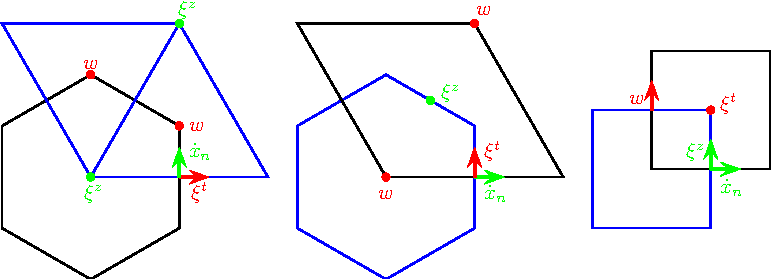
\includegraphics{fig_vortex_boxes.pdf}
\end{center}
\caption{Grid structure for the vortex bracket. The two sketches to the left 
are the top views for the triangular and the hexagonal option, the right sketch
represents the side view. Main boxes are indicated with blue lines and secondary
boxes with black lines. The main vertical layer variables are marked green and 
the top interface variables red.}
\label{heli_grid}
\end{figure}

The vortex bracket is defined according to N\'evir (1998) as
\begin{equation}
\{\mathcal{F},\mathcal{H}\}_{\mathbf{v}}=
-\int_V\frac{\delta\mathcal{F}}{\delta\mathbf{v}}\cdot
\left(\frac{\vec{\omega}_a}{\varrho}\times
\frac{\delta\mathcal{H}}{\delta\mathbf{v}}\right)d\tau,
\label{vortex_bra}
\end{equation}
where $\vec{\omega}_a$ is the absolute vortex vector. The numerical 
discretisation of that bracket turns out to be tricky. The scalar triple 
product may only be computed if the vectors are all reconstructed at the same 
positions in the grid. Because the compliance with the full two-fold 
antisymmetry of the scalar triple product requires an overwhelming amount of 
reconstructions and averagings, we restrict ourselves to the case, when only 
$\mathcal{F}$ and $\mathcal{H}$ permute, which gives at least energy 
conservation. This is in accordance with physical reasoning, which states that 
the full two-fold antisymmetry of a helicity bracket is not needed in 
compressible flows, helicity is not conserved in this case.

For the hexagonal grid, the vector reconstruction procedure for the vorticity
flux term, which is one part of the vortex bracket, was for a long time in the 
history unclear until Thuburn (2008) could show how it must be defined in a 
linearised sense on an equilateral grid. But still, such kinds of 
reconstructions were obtained without employing any kind of bracket philosphy. 
As Thuburn's reconstruction proved as the unique possiblitity to obtain 
undisturbed wave propagation, it must be recovered when linearizing an 
eventually found bracket discretisation.

Before we devote ourselves to the reconstruction of the velocity, we
decompose the problem into two parts, were we distinguish the vertical and the
horizontal vortex vector parts. Formally, we rewrite (\ref{vortex_bra}) as
\begin{equation}
\{\mathcal{F},\mathcal{H}\}_{\mathbf{v}}=
-\int_V\frac{\delta\mathcal{F}}{\delta\mathbf{v}}\cdot
\left(\frac{\xi_{h,a}\mathbf{e_h}}{\varrho}\times
\frac{\delta\mathcal{H}}{\delta\mathbf{v}}\right)d\tau
-\int_V\frac{\delta\mathcal{F}}{\delta\mathbf{v}}\cdot
\left(\frac{\xi_{z,a}\mathbf{e_z}}{\varrho}\times
\frac{\delta\mathcal{H}}{\delta\mathbf{v}}\right)d\tau.
\label{sep_vortex_bra}
\end{equation}
Applying this separation to our discretised problem, we find that the vertical vorticity part asks for horizontal vector reconstructions on a
triangular, quadrilateral or hexagonal mesh, whereas the horizontal vorticity
part considers vertical slices which deal always with some kind of quadrilateral mesh.

Generally, the scalar triple product evaluation might be cast in either of the three coordinate systems: orthogonal, contravariant or covariant. As the vorticities come naturally with contravariant measure numbers and the vortex term generates the vorticity
flux term in a further derivable vorticity equation, where the contravariant fluxes
are needed, one is tempted to pose the problem with covariant base vectors. On the other
hand, the reconstruction of vectors gathers different local coordinate systems with different orographic slopes, so that is it not straightforward to select an actual coordinate system for the reconstructed vectors. Therefore, the evaluation of the of the
vortex bracket is done in the orthogonal system and the vorticities are first transformed
into the orthogonal components.


\subsection{Horizontal vorticity part}
The horizontal vorticity part is discretised in a vertical plane, as given
in the right panel of Figure \ref{heli_grid}. As the tangential vorticity
component is automatically given at the vertical interface points $l$, we
rewrite the vortex backet part as
\begin{displaymath}
 \{\mathcal{F},\mathcal{H}\}_{\mathbf{v}}=...
-\sum_{j,l}\frac{\delta\mathcal{F}}{\delta\mathbf{v}}_{j,l}\cdot
\left(\frac{\xi_{t,a,j,l}\mathbf{e_{t,j,l}}}
{\overline{\overline{\varrho}^j}^l}\times
\frac{\delta\mathcal{H}}{\delta\mathbf{v}}_{j,l}\right)V_{j,l}
\end{displaymath}
Due to the orthogonality of the coordinate system, and the fact, that all
horizontal velocity vector components are given as normal components on the
grid, we find two possible cases for the scalar triple product, which do not
vanish
\begin{eqnarray*}
  a)&&-\mathbf{e_{n;j}}\cdot(\mathbf{e_{t;j}}\times\mathbf{e_z})=
      -\mathbf{e_{n;j}}\cdot\mathbf{e_{n;j}}=-1\\
  b)&&-\mathbf{e_z}\cdot(\mathbf{e_{t;j}}\times\mathbf{e_{n;j}})=
     \mathbf{e_{t;j}}\cdot\mathbf{e_{t;j}}=1,
\end{eqnarray*}
The vector reconstruction is obtained as an volumar weighting of the components
in the box over which $\xi_t$ is defined. The quadrature points for the
reconstruction have to be exactly those, which enter the evaluation of
$\xi_t$. As one can show, only this measure prevents the occurence of a symmetric internal
instablility (Hollingsworth et al., 1983). Thus, we define the discretised bracket as
\begin{eqnarray*}
 \{\mathcal{F},\mathcal{H}\}_{\mathbf{v}}&=&...
-\sum_{j,l}\frac{1}{\sqrt{g}_{j,l}A_{e,j,l}}\sum_{k \in l}\frac{\sqrt{g}_{k,j}}{2}A_{e,j,k}
\frac{\delta\mathcal{F}}{\delta\dot{x}_{n,j,k}}\mathbf{e_n}\cdot\\
&&\left(\frac{\xi_{t,a,j,l}}
{\overline{\overline{\varrho}^j}^l}\mathbf{e_t}\times
\frac{1}{\sqrt{g}_{j,l}dq^{n,j,l}}\sum_{i\in j}\sqrt{g}_{i,l}\widetilde{dq}^{n,i(j),l}
\frac{\delta\mathcal{H}}{\delta w}_{i,l}\mathbf{e_z}\right)\sqrt{g}_{j,l}A_{e,j,l}\\
&&
-\sum_{j,l}\frac{1}{\sqrt{g}_{j,l}dq^{n,j,l}}\sum_{i\in j}
\sqrt{g}_{i,l}\widetilde{dq}^{n,i(j),l}\frac{\delta\mathcal{F}}{\delta w}_{i,l}\mathbf{e_z}
\cdot\\
&&\left(\frac{\xi_{t,a,j,l}}{\overline{\overline{\varrho}^j}^l}\mathbf{e_t}\times
\frac{1}{\sqrt{g}_{j,l}A_{e,j,l}}\sum_{k \in l}\frac{\sqrt{g}_{k,j}}{2}A_{e,j,k}
\frac{\delta\mathcal{H}}{\delta\dot{x}_{n,j,k}}\mathbf{e_n}\right)\sqrt{g}_{j,l}A_{e,j,l}.
\end{eqnarray*}
Here, the usual averaging rules (\ref{avel}) and (\ref{avej}) are again used. The tendency
for the horizontal velocity equation for $\mathcal{F}=\dot{x}_{n,j1,k1}$ reads then using (\ref{avek})
\begin{displaymath}
 \frac{\partial\dot{x}_{n,j1,k1}}{\partial t}=
...-\overline{\overline{\overline{\varrho}^lw}^j
\frac{\xi_{t,a,j,l}}{\overline{\overline{\varrho}^j}^l}}^k_{j1,k1}.
\end{displaymath}
Similarly, the tendency for the vertical velocity tendency equation for $\mathcal{F}=w_{i1,l1}$ yields
\begin{displaymath}
 \frac{\partial w_{i1,l1}}{\partial t}=...
\frac{1}{A_{i1,l1}}\sum_{j\in i1}\widetilde{dq}^{n,j(i1),l1}dq^{t,j,l1}
\left(\overline{\overline{\varrho}^j\dot{x}_{n}}^l\frac{\xi_{t,a,j,l}}{\overline{\overline{\varrho}^j}^l}\right)_{j,l1}.
\end{displaymath}

\subsection{Vertical vorticity part}
The vertical vorticity part is different for the possible horizontal grids in ICON, because
the vorticity resides naturally at different positions. As already mentioned, to avoid the
Hollingsworth instability, the vector reconstructions should use the same points which are
used in the computation of the vertical vorticity, and the stencil of the kinetic
energy discretisation must be appropriately chosen with an approximately similar number of
grid points. Thus, we distinguish three possible cases in ICON
\begin{itemize}
\item{\bfseries Triangular grid.} The dual grid on which the vorticity resides is hexagonal/pentagonal grid.
\item{\bfseries Quadrilateral grid.} The dual grid on which the vorticity resides is a quadrilateral grid.
\item{\bfseries Hexagonal grid.} The dual grid on which the vorticity resides is a rhomboidal grid. This seems not to suit to the general conception, that the dual of a
hexagon is a triangle. But changing the viewpoint to the focus on the trivariate coordinate
system, which spans the hexagonal grid, it is obvious that there are three possibilities
to represent the vorticity, which are identical in the continuous equations, because the
constraints are met which restrict the overspecified coordinate system. If those vorticities
are discretised, they come to lie on the edges of the hexgons in the center of rhombi.
The reconstruction of the velocities again is needed on the same stencil as the vorticities
are defined, but additionally, vector reconstructions on hexagons are needed to match with
the constrains of the trivariate overspecified coordinate system.
\end{itemize}
We first consider the general case, in which the vector reconstruction and the vorticity
are defined on the dual grid. The scalar triple product accounts for
\begin{displaymath}
 -\mathbf{e_{n,j1}}\cdot(\mathbf{e_z}\times\mathbf{e_{n,j2}})=
  \mathbf{e_{n,j1}}\cdot\mathbf{e_{t,j2}},
\end{displaymath}
where the edges $j1$ and $j2$ are to be found at different locations and the belonging
local orthogonal coordinate systems have different orientations so that a vector projection
has to be performed. The natural position for the vorticity is on the dual point $m$ on the
main level $k$. The vortex backet reads now
\begin{eqnarray}
 \{\mathcal{F},\mathcal{H}\}_{\mathbf{v}}&=&...-\sum_{m,k}
\frac{1}{A_{m,k}\sqrt{g}_{m,k}}\sum_{j\in m} dq^{n,j,k}\widetilde{dq}^{t,j(m),k}
\sqrt{g}_{j,k}\frac{\delta\mathcal{F}}{\delta\dot{x}_{n,j,k}}\mathbf{e_{n,j}}
\label{vert_bracket}
\\&&
\cdot\left(\frac{\xi_{z,a,m,k}}{\overline{\varrho}^m}\mathbf{e_z}\times
\frac{1}{A_{m,k}\sqrt{g}_{m,k}}\sum_{j\in m} dq^{n,j,k}\widetilde{dq}^{t,j(m),k}
\sqrt{g}_{j,k}\frac{\delta\mathcal{H}}{\delta\dot{x}_{n,j,k}}\mathbf{e_{n,j}}
\right){A_{m,k}\sqrt{g}_{m,k}}\nonumber
\end{eqnarray}
Inserting now $\mathcal{F}=\dot{x}_{n,j1,k1}$ into the vortex bracket, we find
immediately
\begin{eqnarray*}
 \frac{\partial \dot{x}_{n,j1,k1}}{\partial t}&=&...
\frac{1}{dq^{t,j1,jk}}\sum_{m\in j1}\widetilde{dq}^{n,m(j),k}
\frac{\xi_{z,a,m,k}}{\overline{\varrho}^m}
\mathbf{e_{n,j1}}\cdot\\&&
\left(
\frac{1}{A_{m,k1}\sqrt{g}_{m,k1}}\sum_{j\in m} dq^{n,j,k1}\widetilde{dq}^{t,j(m),k1}
\sqrt{g}_{j,k1}\overline{\varrho}^j_{j,k1}\dot{x}_{n,j,k1}\mathbf{e_{t,j}}
\right).
\end{eqnarray*}

In case of the hexagonal grid, we encounter the fact, that three vorticities are defined
on the grid. They cover rhombi which are each formed by a pair out of the three coordinate
lines. Thuburn (2008) could show, that only a special form of vector reconstruction could
deliver an acceptable form of the dispersion relation for inertial gravity waves. We
find that a certain form of the vortex bracket can recover this rule if linearized. It reads
\begin{eqnarray*}
 \{\mathcal{F},\mathcal{H}\}_{\mathbf{v}}=
\frac{1}{2}\{\mathcal{F},\mathcal{H}\}_{\mathbf{v},hexagon}
+\frac{1}{6}\{\mathcal{F},\mathcal{H}\}_{\mathbf{v},rhombus},
\end{eqnarray*}
where the bracket for the rhombi is evaluated as given in (\ref{vert_bracket}). The edges
which are comprised in one rhombus are those of the two triangles that form the rhombus.
Thus, the edge summation $j\in m$ counts 6 edges. The hexagonal bracket $\{\mathcal{F},\mathcal{H}\}_{\mathbf{v},hexagon}$ differs from the rhombus bracket,
because there is no vorticity defined in the center of the hexagon. To account for
energy conservation which is achieved by the permutability of $\mathcal{F}$ and
$\mathcal{F}$ in the bracket, we divide the hexagon bracket into two parts
\begin{eqnarray*}
 \{\mathcal{F},\mathcal{H}\}_{\mathbf{v},hexagon}&=&...-\frac{1}{2}\sum_{m,k}
\frac{1}{A_{m,k}\sqrt{g}_{m,k}}\sum_{j\in m} dq^{n,j,k}\widetilde{dq}^{t,j(m),k}
\sqrt{g}_{j,k}\frac{\delta\mathcal{F}}{\delta\dot{x}_{n,j,k}}
\frac{\xi_{z,a,j,k}}{\overline{\varrho}^j}
\mathbf{e_{n,j}}
\\&&
\cdot\left(\mathbf{e_z}\times
\frac{1}{A_{m,k}\sqrt{g}_{m,k}}\sum_{j\in m} dq^{n,j,k}\widetilde{dq}^{t,j(m),k}
\sqrt{g}_{j,k}\frac{\delta\mathcal{H}}{\delta\dot{x}_{n,j,k}}\mathbf{e_{n,j}}
\right){A_{m,k}\sqrt{g}_{m,k}}\\
&&-\frac{1}{2}\sum_{m,k}
\frac{1}{A_{m,k}\sqrt{g}_{m,k}}\sum_{j\in m} dq^{n,j,k}\widetilde{dq}^{t,j(m),k}
\sqrt{g}_{j,k}\frac{\delta\mathcal{F}}{\delta\dot{x}_{n,j,k}}
\mathbf{e_{n,j}}
\\&&
\cdot\left(\mathbf{e_z}\times
\frac{1}{A_{m,k}\sqrt{g}_{m,k}}\sum_{j\in m} dq^{n,j,k}\widetilde{dq}^{t,j(m),k}
\sqrt{g}_{j,k}\frac{\delta\mathcal{H}}{\delta\dot{x}_{n,j,k}}
\frac{\xi_{z,a,j,k}}{\overline{\varrho}^j}\mathbf{e_{n,j}}
\right){A_{m,k}\sqrt{g}_{m,k}},
\end{eqnarray*}
where the vorticity contribution is once used in connection with $\mathcal{F}$ and
another time in connection with $\mathcal{H}$. Consequently, by permuting $\mathcal{F}$
and $\mathcal{H}$ the antisymmetry of the bracket is guaranteed. One could have used
this very approach also in the rhombus bracket. Experimentation with the hydrostatic
model suggests that this alternative is not as stable as the method documented here. The
reason seems to be related to the occurence of the Hollingsworth instability. This
instability can probably not be prevented completely, but the current version performs
best under all methods tested so far (which were: (i) use the hexagon bracket approach
also for the rhombus brackets, (ii) average 6 rhombus vorticities to the center of the
hexagon and use the hexagon bracket similarly to the rhombus bracket).

